\medskip
\noindent\textbf{Proposta de Valor}\\
O sistema tem como objetivo central ajudar os agricultores a identificarem deficiências de manganês e cobre nas folhas de mexerica, contribuindo para manter o padrão de qualidade da fruta. A utilização de inteligência artificial integrada ao sistema oferece precisão na análise das fotos enviadas pelos usuários.

\medskip
\noindent\textbf{Segmento de Mercado}\\
O público-alvo são os agricultores de mexerica do Vale do Ribeira, com foco específico em produtores rurais, horticultores e demais interessados na melhoria da produtividade agrícola.

\medskip
\noindent\textbf{Relacionamento com o Cliente}\\
O relacionamento com os usuários será realizado via WhatsApp, aplicativo móvel e site institucional. Os usuários poderão enviar fotos das folhas e receber feedback automatizado por meio de gráficos e mapas gerados pelo sistema. O aplicativo também permite o envio de análises e resultados personalizados.

\medskip
\noindent\textbf{Canais}\\
A divulgação e o acesso ao sistema ocorrerão por meio de anúncios em secretarias de agricultura dos municípios da região, com suporte adicional via site, e-mail e WhatsApp da empresa, fortalecendo a comunicação direta com o público-alvo.

\medskip
\noindent\textbf{Atividades-Chave}\\
As principais atividades envolvem a identificação de deficiência nutricional nas folhas e o fornecimento de suporte técnico e manutenção contínua do sistema.

\medskip
\noindent\textbf{Recursos-Chave}\\
Para operar corretamente, o sistema depende de uma equipe técnica composta por programadores, instaladores do sistema físico e profissionais responsáveis pelo suporte online. Além disso, é necessário um serviço de hospedagem para o site e para o banco de dados.

\medskip
\noindent\textbf{Parcerias-Chave}\\
As parcerias incluem associações de fazendeiros, secretarias de agricultura locais e participação em feiras do setor agrícola, que auxiliam na disseminação e na credibilidade do projeto.

\medskip
\noindent\textbf{Estrutura de Custos}\\
Inclui gastos com manutenção dos equipamentos de monitoramento, aluguel de espaço físico para atendimento, aquisição de materiais e tecnologias para análise das folhas, além de custos com servidores para armazenamento dos dados.

\medskip
\noindent\textbf{Fontes de Renda}\\
A monetização ocorre por meio do aluguel do sistema, da cobrança pelo aluguel de equipamentos necessários e da prestação de serviços de instalação e manutenção.
\medskip

\begin{figure}[H]
\centering
\caption{Modelo de Negócios Canvas}
\label{fig:Canvas}
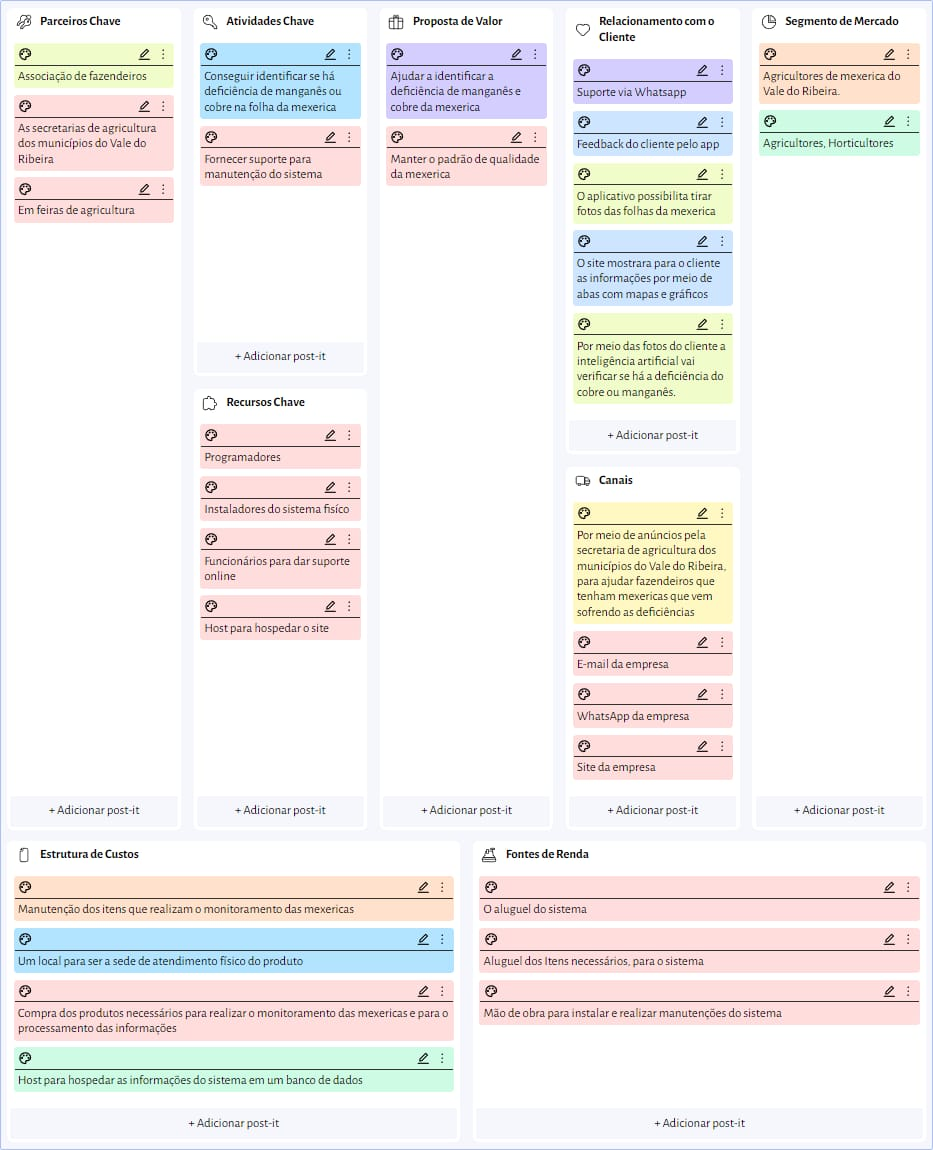
\includegraphics[width=0.8\textwidth]{Images/Canvas.jpeg}
\SourceOrNote{Equipe 21 - Vitalliz (2025)}
\end{figure}
\medskip